\begin{frame}{Representação Intermediária de Código}
    \begin{itemize}
        \item Estrutura de dados usada para manter integridade semântica e possibilitar otimizações~\cite{cooper2014}
              \begin{itemize}
                  \item[--] Classificadas de acordo com o nível de abstração
                  \item[--] Muitas vezes aplicadas em sequência
              \end{itemize}
        \item[] \begin{figure}
                  \centering
                  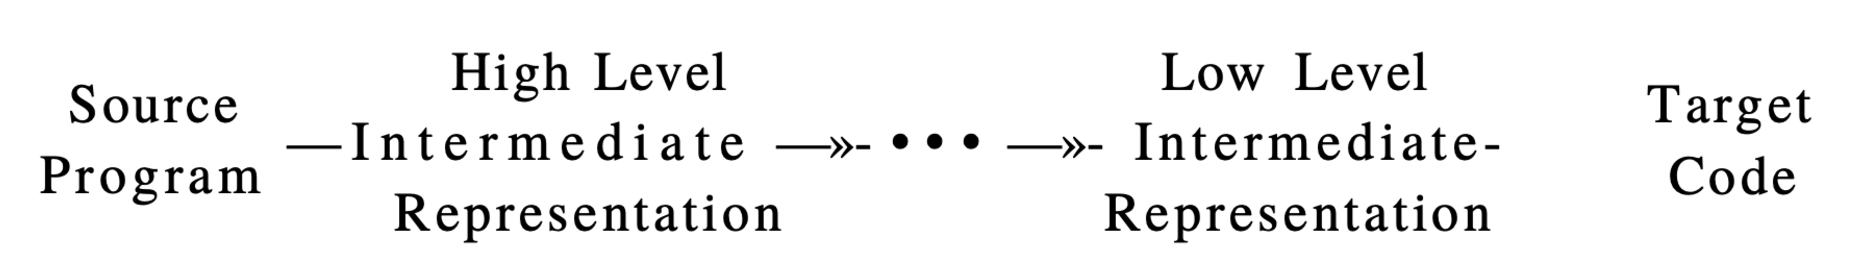
\includegraphics[width=.7\textwidth]{Imagens/abstraction-level-irs.eps}
                  \caption{Sequência de representações intermediárias}\label{fig:abstraction-level-irs}
                  \small{Fonte:~\cite{aho2008compilers}}
              \end{figure}
        \item Fluxo de controle
              \begin{itemize}
                  \item[--] Ordem das instruções
                  \item[--] Escopo
              \end{itemize}
    \end{itemize}
\end{frame}
